\chapter{Unidad de Procesamiento de Graficos de Proposito General}
\spacing{1.5}
"Las GPU han evolucionado al punto que muchas aplicaciones del mundo real se están implementando fácilmente en ellas y se ejecutan muchísimo más rápido que en sistemas con múltiples núcleos. Las arquitecturas de computación del futuro serán sistemas híbridos con GPU de núcleos paralelos trabajando en tándem con CPU de múltiples núcleos" (figura 3-1).\cite{GPUIntro}
\begin{figure}[H]
                      \centering
                              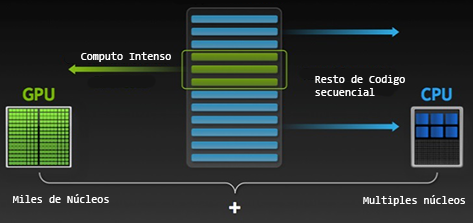
\includegraphics[height=6cm]{img/how-gpu-acceleration-works.png}
                      \caption{Sistema Híbrido con GPU y CPU}
\end{figure}
\section{Breve Historia de las GPU}
La necesidad de mejorar los gráficos para los videojuegos provocó un gran avance en el diseño de hardware. En la década de los ochentas las tarjetas gráficas dedicadas, no eran más que pipelines fijos que desplegaban formas geométricas calculadas por el CPU por medio del hardware de acceso directo a memoria (DMA). Esto les daba un funcionamiento fijo y solo eran configurables mediante dos librerías: OpenGL de \textit{Silicon Graphics} y Direct3D de \textit{Microsoft}.\\
A finales de los noventas el hardware se volvió más programable, un ejemplo de estas tarjetas gráficas es la GeForce 256\cite{GeForce256} fue lanzada al mercado en 1999, a la que se le acuño el nombre de GPU. La cual aportó características graficas importantes, como por ejemplo: funciones de  transformación, iluminación, organización y rendering, la capacidad de procesar 15 millones de triángulos por segundo y un rendimiento de 480 millones de píxeles por segundo. Además su motor de rendering  256 bits mostró una mejora en cuanto a la complejidad visual.\\
Esta tecnología revolucionaria llamó la atención de otros profesionales, además de artistas y desarrolladores de vídeo juegos, quienes utilizaron el gran rendimiento de punto flotante que tenían los GPU para otros objetivos por ejemplo procesar imágenes médicas, exploración sísmica, centros de supecómputo, entre otras\cite{aplicaciones}. De esta forma surge un movimiento para utilizar para fines diferentes a los gráficos a las GPU.\\
En ese momento, la GPU de propósito general (GP-GPU) era muy difícil de manipular: solo aquellos que tenían amplios conocimientos en lenguajes de programación de gráficos desarrollaban para estas plataformas. Puesto que los cálculos para resolver los problemas generales debían ser representados por triángulos o polígonos.\\
Fue hasta 2001, en la Universidad de Stanford, cuando un equipo liderado por Ian Buck se propuso ver el GPU como un  \textit{procesador de flujos}. Este equipo desarrollaría \textit{Brook} \cite{Buck2001}, un lenguaje de programación diseñado para tener la misma sintaxis de C, con algunas características adicionales. Y con el objetivo de minimizar el complejo trabajo de análisis que se requería para generar aplicaciones paralelas. En este, se introdujeron  conceptos como los flujos (streams), kernels y los operadores de reducción. Esto generó un gran impulso a los GPU como procesadores de propósitos generales, principalmente por dos razones: pues se trataba de un lenguaje de más alto nivel. Lo más importante, los programas escritos en \textit{Brook} eran hasta 7 veces más rápido que códigos similares existentes.\\
La compañía NVIDIA se dio cuenta que tenía un hardware muy poderoso en las manos, sin embargo debía complementarlo con herramientas de hardware y software intuitivas. Invitó a Ian Buck a colaborar con ellos. El objetivo sería ejecutar C a la perfección en una GPU. NVIDIA alcanzó este objetivo en 2006 con el lanzamiento de CUDA, la cual sería la primera solución para las GP-GPU. Aunado a esta solución, lanzó la GeForce 8800, la cual fue diseñada para ser usada en cómputo de propósito general con su arquitectura inspirada en la de CUDA.
\section{Plataforma y modelo de programación de cómputo paralelo}
NVIDIA lanzó en noviembre de 2006 una Arquitectura Unificada de Dispositivos de Cómputo (CUDA), es una plataforma para cómputo paralelo y un modelo de programación, que permite obtener aumentos en los rendimientos del cómputo gracias a la ayuda que la unidad de procesamiento de gráficos le proporciona al CPU. \\
Los dispositivos CUDA aceleran la ejecución de los programas que procesan una gran cantidad de datos ya que la arquitectura de esta plataforma, es similar a un procesador tradicional de computadora pero, tienen la cualidad de que los procesadores son masivamente paralelos, equipados con una gran cantidad de unidades aritméticas. En estas unidades aritméticas se ejecuta la misma instrucción y de acuerdo con la taxonomía de Flynn, pertenecen a la categoría de \textit{una instrucción, múltiples datos} (SIMD) como se puede ver en la figura 3-2.\\ 
\begin{figure}[H]
                      \centering
                              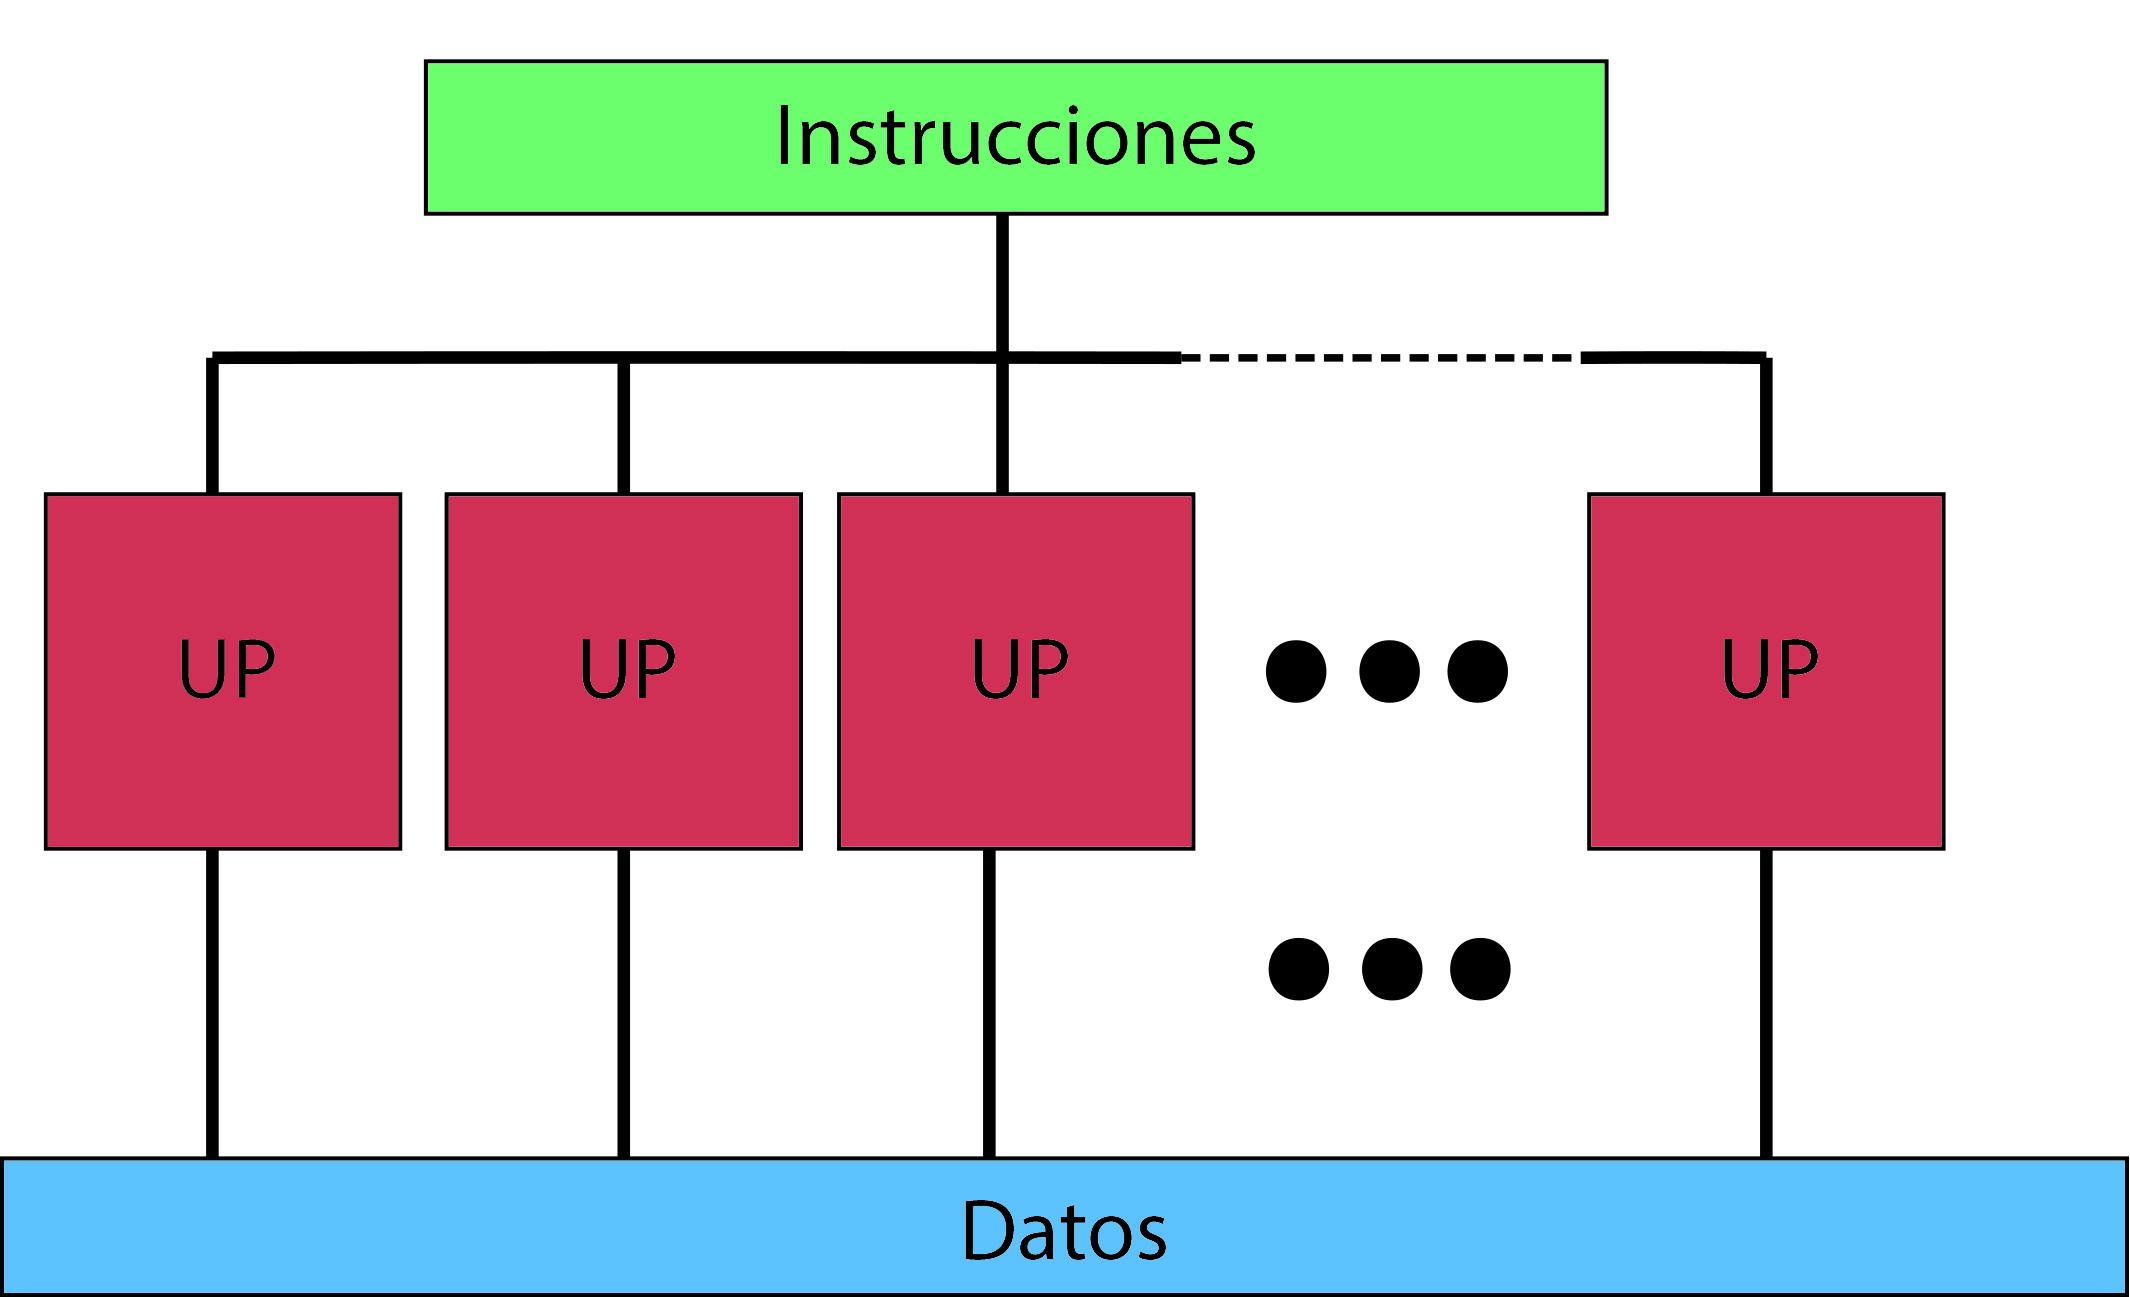
\includegraphics[height=5cm]{img/SIMD.jpg}
                      \caption{SIMD}
\end{figure}
El modelo de programación para desarrollar programas para las GPU, es una extensión del lenguaje C conocida como CUDA C. Actualmente existen alternativas a CUDA C tales como FORTRAN, Python, .NET (combinando CUDA con Microsoft's F\#), o alguna API como OpenCL u OpenACC\cite{lenguajes}. 
\subsection{Arquitecturas}
Como se describió anteriormente la arquitectura de CUDA fue diseñada para que la GPU pudiera ser utilizada en aplicaciones de propósito general. Ésta tiene un arreglo de procesadores con múltiples unidades aritmético-lógicas (ALU), las cuales fueron diseñadas para poder realizar operaciones de punto flotante, cumpliendo los requisitos del Instituto de Ingeniería Eléctrica y Electrónica (IEEE). Además de esto, las ALU deben tener acceso a diferentes tipos de memoria, como la compartida entre unidades y la memoria de la tarjeta gráfica.\\
Estas ALU tan particulares en la arquitectura de CUDA se conocen como \textit{CUDA cores} y conforman gran parte de los Streaming Multiprocessor (SM). Los SM son procesadores que tienen la tarea de ejecutar los hilos concurrentemente. Además, los CUDA cores están formados por una memoria cache (shared memory), registros y unidades de funciones especiales.
\subsubsection{Arquitectura Fermi}
Los GPU basados en la arquitectura Fermi \cite{fermi}, están formados por 512 CUDA cores. Los CUDA cores ejecutan operaciones de punto flotantes o enteras por ciclo de reloj en cada hilo. Los 512 CUDA cores están organizados en 16 SM de 32 cores cada uno (figura 3-3). El GPU tiene seis particiones de memoria de 64-bits, una capacidad de leer 384-bits de la memoria simultáneamente y una capacidad de hasta 6GB de memoria DRAM categoría DDR5. El sistema de conexión entre el GPU y el CPU es vía PCI-Express. La forma en que se hace la distribución del trabajo en cada bloque es decidida por el módulo llamado \textit{GigaThread}, el cual pasa las tareas a cada SM para que  haga la asignación de trabajo a cada hilo.\\

\begin{figure}[H]
                      \centering
                              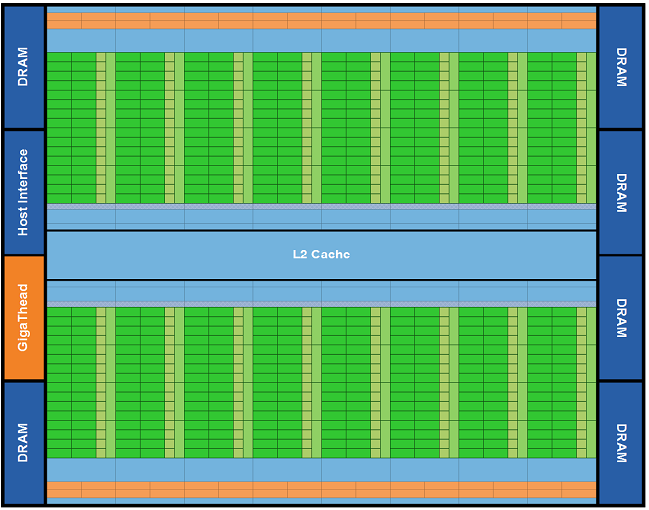
\includegraphics[height=10cm]{img/ArqFermi.png}
                      \caption{La arquitectura Fermi tiene sus 16 SM alrededor de la memoria compartida L2 cache \cite{fermi} Ver figura 3-4 para detalle de los SM.}
\end{figure}
Esta arquitectura tiene cualidades significativas como el rendimiento en las operaciones de doble precisión dedicado a cómputo científico, soporte para corrección de errores para asegurar las operaciones con números muy grandes en aplicaciones delicadas. Se implementó una jerarquía en la memoria cache que permitió aumentar la eficiencia en cuanto a las  lecturas a memoria, la memoria compartida tuvo un incremento y las operaciones atómicas incrementaron su desempeño gracias a que se aumentaron las unidades de operaciones atómicas y la aparición de la memoria cache L2.\\
Las SM de la arquitectura Fermi (figura 3-4) están formadas por diferentes elementos, iniciando por los 32 CUDA cores, cada uno con una unidad aritmética lógica para las operaciones con enteros y una unidad de punto flotante. Cumplen con la norma IEEE 754-2008 que permite realizar una multiplicación y una suma en un solo paso de redondeo. La asignación de trabajo en las SM se realiza por el modulo \textit{GigaThread}, que divide en bloques de hilos a cada SM. Después los planeadores de \textit{warps} dividen el trabajo de este bloque en grupos de 32 hilos para su ejecución dentro de la SM. Cuentan también con 16 unidades load/store, las cuales permiten calcular el origen y destino de los dieciséis hilos por pulso de reloj, y 4 unidades de funciones especiales (SFU), que ejecutan instrucciones complejas como cálculo de senos, cosenos, reciproco y raíz cuadrada. 
\begin{figure}[H]
                      \centering
                              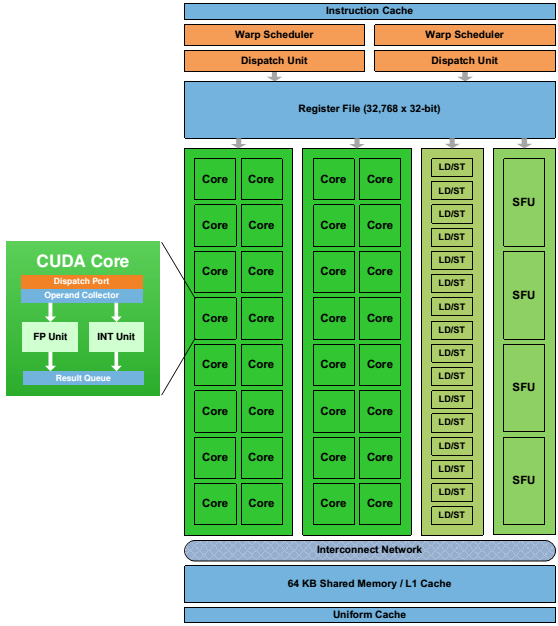
\includegraphics[height=15cm]{img/fermiSM.png}
                      \caption{Fermi Streaming Multiprocessor (SM)\cite{fermi}}
\end{figure}
\subsubsection{Arquitectura Kepler}
La arquitectura Kepler \cite{Kepler}, modificó los SM de su antecesor Fermi llamándolo Next Generation Streaming Multiprocessor (SMX) (figura 3-5). El nuevo procesador de esta arquitectura está formado por 15 de estos procesadores y 6 controladores de memoria de 64-bits.La cantidad de CUDA cores que contiene es de 192 de precisión simple, y 64 unidades de doble precisión.\\
\begin{figure}[H]
                      \centering
                              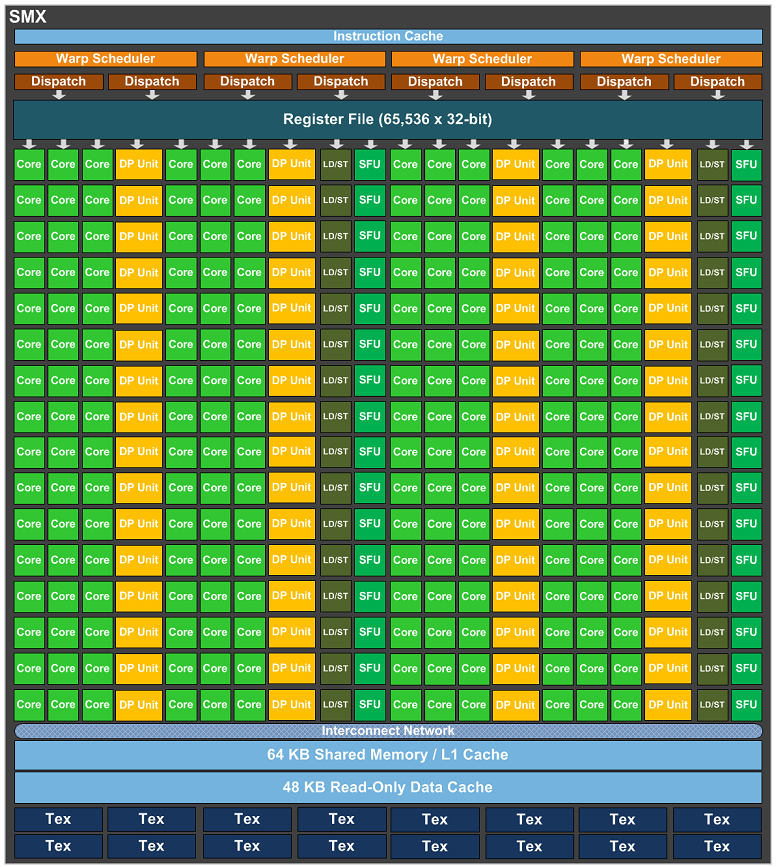
\includegraphics[height=16cm]{img/KeplerSMX.png}
                      \caption{Kepler Next Generation Streaming Multiprocessor (SMX) \cite{Kepler}}
\end{figure}
Las unidades load/store aumentaron a 32 y las SFU incrementaron a 32, ocho veces más que en la Fermi. La asignación de tareas a hilos dentro del SMX es un trabajo desempeñado por los planeadores de warps, los cuales cuenta con bloques de 32 hilos. Además, tiene 4 planificadores de warps, por lo que se tienen 2 unidades de despacho de instrucciones, las cuales permiten  repartir y ejecutar los 4 warps de manera concurrente.\\
También cuenta con una memoria caché L1 con una capacidad de 64KB, configurable a 16, 32 o 48 KB para la memoria cache y el resto para la memoria compartida. Esto da 65536 registros por SMX, en los cuales, cada hilo puede tener acceso a 255 registros para el almacenamiento de datos. Integra una memoria de textura, la cual es un recurso valioso para programas donde se requiere probar o filtrar datos de una imagen. La memoria de textura en esta arquitectura dejó de ser un hardware dedicado solo a este objetivo y se creó un espacio en la memoria global de solo lectura de 48KB que funciona como una memoria caché para agilizar las lecturas.\\
En esta arquitectura se agregó una característica: no se requiere del CPU para lanzar programas en la GPU, es decir, la GPU tiene la capacidad de generar más carga de trabajo, administrar recursos y obtener resultados dentro de la misma GPU (en la zona de más interés), donde se pueda requerir más poder de cómputo.
\subsubsection{Arquitectura Maxwell}
La arquitectura Maxwell\cite{Maxwell}, sufrió un cambio de diseño para aumentar drásticamente su desempeño. Entre sus cambios, se tienen los nuevos SM llamados SM Maxwell (SMM) (figura 3-6), se redujo el número de CUDA cores a 128 y se separaron en 4 divisiones de 32. Cada una de esas divisiones tiene un planificador de warps para su bloque, el cual es capaz de despachar dos instrucciones por ciclo de reloj. Estas divisiones permitieron que se utilizara de una manera más eficiente el espacio y la energía gastada para el manejo de la transferencia de datos.\\
La memoria compartida se incrementó a 96KB y ya no se compartió con la memoria caché L1. Esta última comparte espacio con la memoria de textura. Los registros, las SFU, y las unidades load/store siguieron siendo la misma cantidad.
\begin{figure}[H]
                      \centering
                              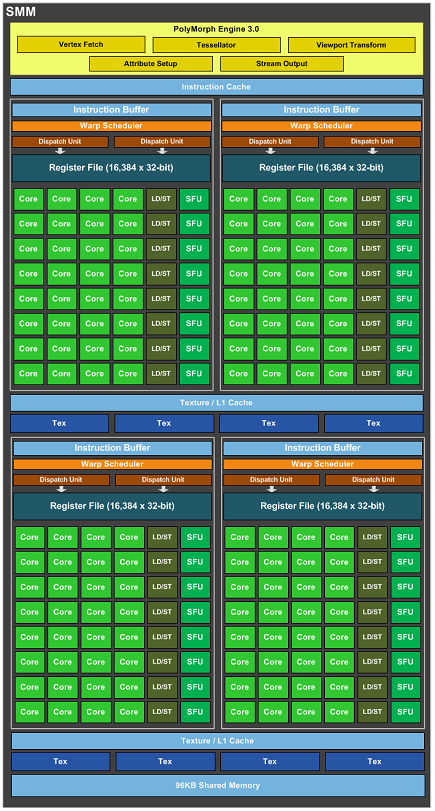
\includegraphics[height=20cm]{img/MaxwellSM.png}
                      \caption{Maxwell Streaming Multiprocessor (SMM) \cite{Maxwell}}
\end{figure}
\section{Modelo de Programación CUDA C}
La extensión del lenguaje C que proporciona CUDA para programar aplicaciones basadas en su arquitectura ofrece a los programadores familiarizados con este lenguaje una manera sencilla de escribir programas para ser ejecutados en la GPU. A continuación se explicará el núcleo del conjunto de instrucciones de esta extensión.
\subsection{Kernels}
CUDA C, permite definir funciones llamadas \textit{kernels} las cuales, cuando son llamadas, se ejecutan N veces en paralelo en N diferentes \textit{hilos} CUDA. Para definir un kernel se usa la declaración \textbf{\_\_global\_\_}. Estos kernels se ejecutan en un dispositivo: la tarjeta gráfica instalada en la computadora, y se invocan por medio del equipo anfitrión. Este anfitrión no es más que el procesador que estará usando la tarjeta gráfica como coprocesador. El siguiente código muestra cómo se declara un kernel: 
\spacing{1.5}
\singlespacing
\lstset{language=C,
                basicstyle=\ttfamily,
                keywordstyle=\color{blue}\ttfamily,
                stringstyle=\color{red}\ttfamily,
                commentstyle=\color{green}\ttfamily,
        frame= none,
        captionpos=b,    
        numbers = left,
        xleftmargin=2em,
        framexleftmargin=1.5em,
        tabsize=2        
}
\begin{lstlisting}[caption=Declaración de un Kernel en CUDA C.]
__global__ void kernel( ... )
{
        ...
}
\end{lstlisting}
\spacing{1.5}
Al lanzar un kernel desde el anfitrión, se debe escoger una configuración para los hilos CUDA que se lanzaran para ejecutarlo, dándole a cada uno de estos un identificador único (\textit{threadID}). 
\subsection{Jerarquía de Hilos}
La configuración que se usa para lanzar los hilos, se especifica entre  \textbf{\textless\textless\textless} y \textbf{\textgreater\textgreater\textgreater}. Se requiere de dos parámetros para el lanzamiento: el primero es la dimensión de la malla (véase figura 3-7), que se refiere al número de bloques, y el segundo es la dimensión del bloque, que es el número de hilos. 
\begin{figure}[H]
                      \centering
                              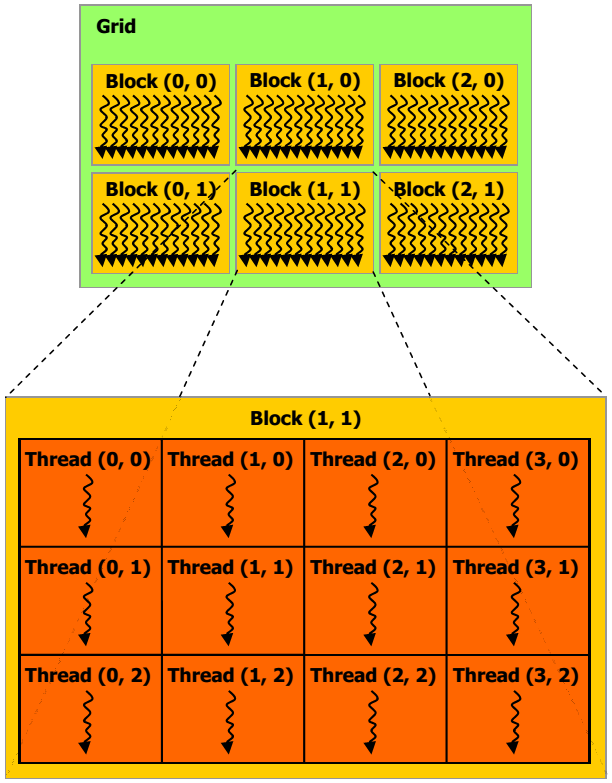
\includegraphics[height=8cm]{img/grid_block.png}
                      \caption{Organización bloques en malla e hilos en bloques \cite{Flops}}
\end{figure}
Cada hilo tiene un identificador al que se puede acceder mediante el identificador  \textbf{threadIdx}, el cual es un vector de tres componentes, por lo que, los hilos pueden usar identificadores de uno, dos o tres dimensiones para formar bloques unidimensionales, bidimensionales o tridimensionales. Los bloques están organizados en una malla que puede tener una, dos o tres dimensiones, y tienen un identificador al cual se puede acceder usando la variable \textbf{blockIdx}. Existe otra variable importante \textbf{blockDim} la cual especifica la dimensión del bloque.\\
A continuación se presenta un ejemplo de cómo se lanza un kernel:
\spacing{1.5}
\singlespacing
\lstset{language=C,
                basicstyle=\ttfamily,
                keywordstyle=\color{blue}\ttfamily,
                stringstyle=\color{red}\ttfamily,
                commentstyle=\color{green}\ttfamily,
        frame= none,
        captionpos=b,    
        numbers = left,
        xleftmargin=2em,
        framexleftmargin=1.5em,
        tabsize=2        
}
\begin{lstlisting}[caption=Lanzamiento de un Kernel en CUDA C.]
__global__ void miKernel( ... )
{
        ...
}
int main(...)
{
        ...     
        dim3 gridDim(...,...,...);
        dim3 blockDim(...,...,...);
        miKernel<<<gridDim,blockDim>>>(...);    
        ...
}
\end{lstlisting}
\spacing{1.5}
Una parte fundamental del paralelismo es la comunicación entre cada proceso/hilo que se ejecuta simultáneamente. Hacer cooperar los hilos en la GPU no es tarea fácil. Para la comunicación entre hilos se tiene la memoria compartida la cual permite el intercambio de datos solo entre hilos del mismo bloque. En cuanto a la sincronización de los hilos, se tiene una función llamada \textbf{\_\_syncthreads()}, la cual sincroniza los hilos por barrera. Esto quiere decir que un hilo no puede seguir ejecutando su tarea hasta que todos los demás hilos lleguen a la misma instrucción. Esta característica solo aplica para  hilos del mismo bloque. En la figura 3-8 se puede observar cómo se asignan los bloques a cada SM. Estos podrían asignarse en cualquier orden y ejecutarse en tiempos diferentes. De este modo, la sincronización de los hilos y la escritura/lectura a memoria compartida se permite, con la característica de que solo los hilos de un mismo bloque pueden ser sincronizados o comunicarse por medio de memoria compartida.
\begin{figure}[H]
                      \centering
                              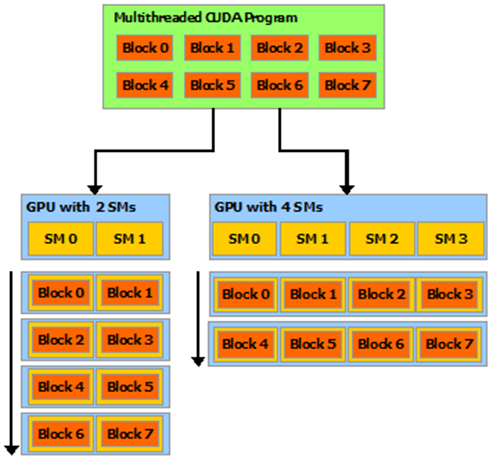
\includegraphics[height=10cm]{img/block_sm.png}
                      \caption{Asignación de bloques por SM \cite{Flops}}
\end{figure}
\subsection{Jerarquía de Memoria}
La arquitectura CUDA cuenta con diferentes tipos de memoria, de los cuales se pueden leer los datos para operar y escribir los resultados obtenidos por los hilos, los cuales, son los encargados de realizar las operaciones sobre los datos. Cada uno de estos bancos de almacenamiento tiene características diferentes que, utilizados adecuadamente, pueden ayudar a mejorar el despeño de los programas. A continuación se hablará de los tipos de memoria que se encuentran en las GPU (figura 3-9).\\
\begin{figure}[H]
                      \centering
                              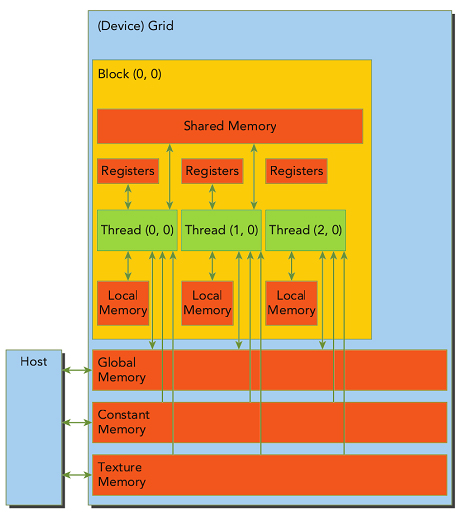
\includegraphics[height=10cm]{img/memoria.jpg}
                      \caption{Tipos de Memoria de la GPU \cite{chengl} }
\end{figure}
Los \textit{registros} son el tipo de memoria con el tiempo de lectura/escritura más rápido en el dispositivo. En cada SM, hay miles de registros y los cuales son asignados en una cantidad fija a cada hilo cuando es lanzado un kernel. Estos son de 32-bits y pueden almacenar datos de tipo flotante o entero. La manipulación de los registros esta administrado por el sistema.\\
La \textit{memoria local} es un espacio de memoria privada que cada hilo tiene. En esta se almacenan los datos que no pudieron ser almacenados en los registros por ejemplo las variables locales, las llamadas a funciones y el contexto de ejecución. Al igual que los registros, esta memoria es administrada por el sistema.\\
La \textit{memoria compartida} es una memoria de tipo caché que se comparte entre hilos de un mismo bloque. Esta permite que los hilos de un bloque puedan comunicarse escribiendo y leyendo en ella para cooperar en la realización de un mismo objetivo. Su caché es especial ya que el programador define su manejo. La forma en la que se declara una variable en este espacio es mediante la palabra reservada \textbf{\_\_shared\_\_}. La latencia en esta memoria es hasta 100 veces menor que en la memoria global.\\
La \textit{memoria constante} es una memoria de solo lectura, la cual alberga datos que no cambian a lo lago de la ejecución del kernel. Se puede usar esta memoria en el dispositivo igual que la memoria global, pero esta optimizada para enviar datos de lecturas a múltiples hilos. Esto se logra gracias a diferentes instrucciones  que permiten el acceso a este cache de una forma más eficiente. Se puede declarar dicha variable con la palabra reservada \textbf{\_\_constant\_\_}, pero su contenido debe ser asignado por el anfitrión en la memoria del dispositivo, antes de lanzar el kernel mediante la función \textbf{cudaMemcpyToSymbol()}.\\
La \textit{memoria de textura}, al igual que la memoria constante, es una memoria de solo lectura. Está diseñada para trabajar con estructuras llamadas CUDA array las cuales permiten lecturas eficientes en arreglos de hasta tres dimensiones. Las lecturas en este tipo de memoria tienen ventajas, como las diferentes formas de acceso o las interpolaciones de los datos, que se pueden utilizar sin costos adicionales de tiempo.\\
La \textit{memoria global} es la memoria de lectura/escritura de mayor capacidad en la tarjeta gráfica, llegando al orden de los gigabytes. Las funciones que tiene son lectura de datos y escritura de resultados. También funciona como interfaz entre la GPU y el CPU. La persistencia de los datos en esta memoria es hasta que se liberen, lo que permite compartir datos entre kernels. Los hilos pueden acceder en cualquier momento a esta, pero su latencia es tan alta que puede provocar que sea más tardada la lectura de datos que los cálculos que se quieren realizar. Las funciones para reservar, manejar y liberar el espacio en memoria, desde el anfitrión, son: \textbf{cudaMalloc()}, \textbf{cudaMemCpy()} y \textbf{cudaFree()}.
\subsection{Programación heterogénea}
Para entender el modelo de programación de CUDA, es pertinente definir que código ejecutará el CPU y que código el GPU, a fin de que estos puedan trabajar en conjunto. El CPU es el equipo anfitrión (Host) el que decidirá cuándo es necesario usar al dispositivo GPU (Device), el anfitrión y el dispositivo también tendrán memorias separadas.Un Programa en CUDA C se ejecuta tal como se muestra en la figura 3-10.\\
\begin{figure}[H]
                      \centering
                              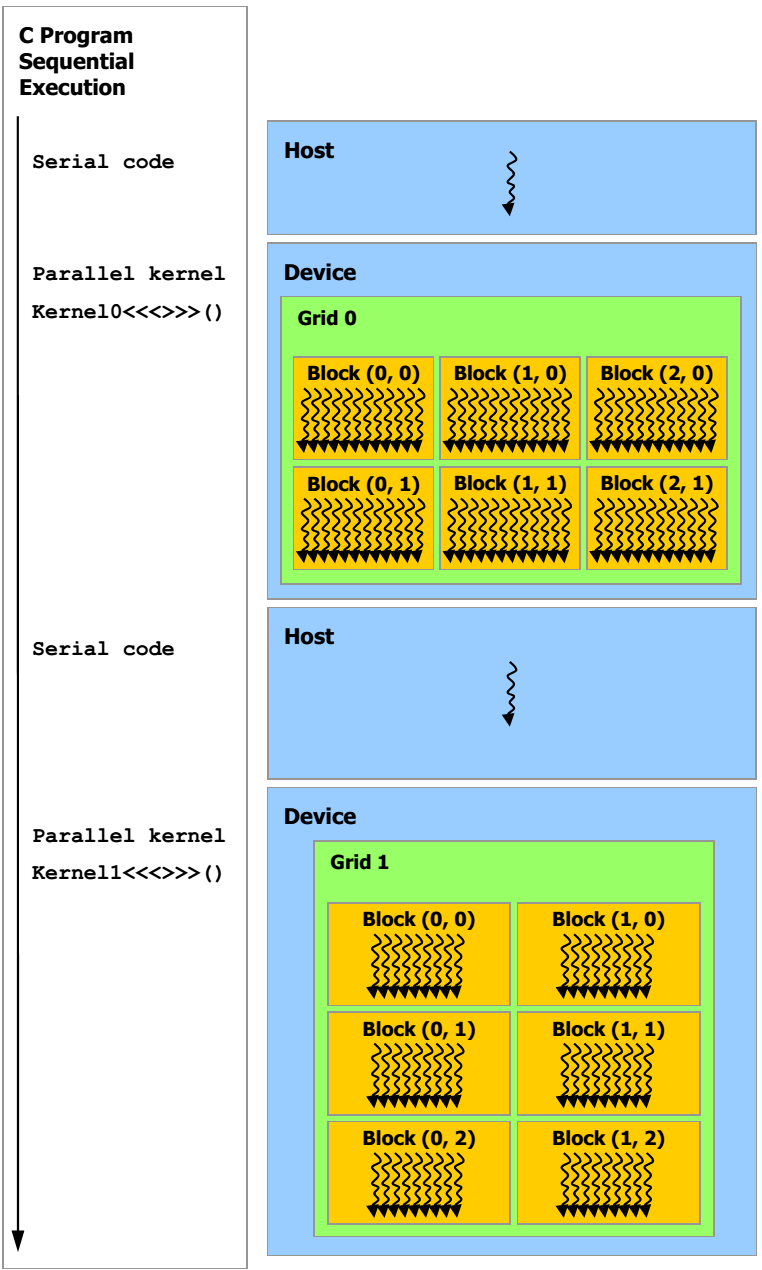
\includegraphics[height=14cm]{img/PH.png}
                      \caption{Programación Heterogénea \cite{Flops}}
\end{figure}
En el código 3.3 de ejemplo se puede ver la estructura básica de un programa, y cómo se declaran y definen funciones kernel. También se puede ver que hay funciones ejecutables en el GPU que son llamadas desde algún kernel definidas con la palabra reservada \textbf{\_\_device\_\_}.\\
En la función principal, el anfitrión se encarga de obtener los datos que se le proporcionaran al kernel y almacenarlos para ser procesados por el  GPU. También se puede ver cómo es que se reserva la memoria en el dispositivo para los datos de entrada y salida que el kernel necesite para procesarlos.\\
Después de realizar una copia de los datos del anfitrión al dispositivo, se pueden ejecutar uno o más kernels en la GPU. Una vez finalizada la ejecución de sus kernels, el resultado se copia a la memoria del anfitrión. Al final, sólo queda liberar los recursos que ya no serán utilizados.
\spacing{1.5}
\singlespacing
\lstset{language=C,
                basicstyle=\ttfamily,
                keywordstyle=\color{blue}\ttfamily,
                stringstyle=\color{red}\ttfamily,
                commentstyle=\color{green}\ttfamily,
        frame= none,
        captionpos=b,    
        numbers = left,
        xleftmargin=2em,
        framexleftmargin=1.5em,
        tabsize=2
}
\begin{lstlisting}[caption=Estructura general de un programa en CUDA C.]
__device__ L funcionDevice()
{ ... } 
__global__ void KernelUno(L*, ... )
{
        ...
        L r= fooDevice();
        ...
}
__global__ void KernelDos( ... )
{ ... }
int main(...)
{       
        ...
        L* datosD;
        cudaMalloc(&datosD,size);
        ...             
        cudaMemcpy(datosD,src,size,cudaMemcpyHostToDevice);             
        ...     
        dim3 gridDim(...,...,...);
        dim3 blockDim(...,...,...);
        KernelUno<<<gridDim,blockDim>>>(datosD,...);    
        ...
        KernelDos<<<...,...>>>(...);
        ...
        cudaMemcpy(res,datosD,size,cudaMemcpyHostToDevice);
        ...
        cudaFree(datosD);
        ...                     
}
\end{lstlisting}
\spacing{1.5}

